\chapter{Implementation}
\label{chap:impl}

In this chapter we describe the internal design of the tokenizer and provide
rationale for the choices behind it. We explore the problem of rough
tokenization more deeply as it posed one of the biggest challenges in building
the system. Finally, we talk about the multi-threading tools which were used to
enable parallelism in the tokenizer.


\section{Overview of the System}
\label{sec:impl-overview}

The data flow between the various subsystems can be seen in
Figure~\ref{fig:all-parts}.

\begin{figure}
  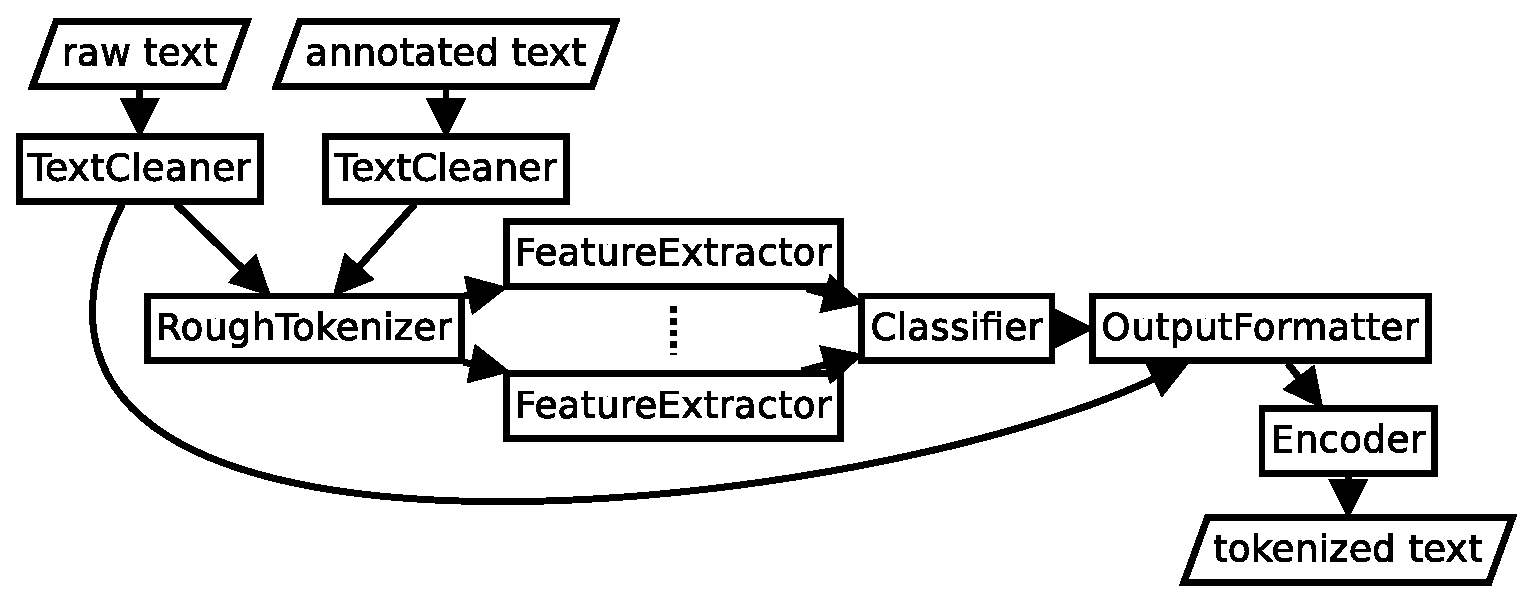
\includegraphics[width=\textwidth]{img/all-parts.eps}
  \caption{Data flow in the entire system}
  \label{fig:all-parts}
\end{figure}

\subsection{TextCleaner}
\label{ssec:impl-overview-textcleaner}

Any input which is read by the tokenizer is first processed with the
\class{TextCleaner}. This unit is responsible for decoding the stream of text
and optionally removing XML markup and expanding HTML entities and character
references. These changes to the input stream (referred to as \newterm{cutouts}
in the program) are conveyed to the \class{OutputFormatter} so that they can be
undone in the output. This allows the tokenizer to process XML marked up
content as if it was plaintext. The XML markup thus cannot be broken by and
does not interfere with the tokenization process.

\subsection{RoughTokenizer}
\label{ssec:impl-overview-roughtokenizer}

The \class{RoughTokenizer}'s goal is to examine the cleaned input stream and
identify both unambiguous and ambiguous token and sentence boundaries. It does
so by splitting the text into what we call \newterm{rough tokens}. In the
simplest case, rough tokens are the whitespace delimited words of the text (the
term \newterm{word} will be used to mean a maximal subsequence of nonwhite
characters). However, the user can write regular expressions to define certain
points within and between these strings of nonwhite characters which may split
them up into what end up being the rough tokens. These user-defined points are
called \newterm{decision points} and they represent the ambiguous
token/sentence boundaries.

There are three types of decision points. There is the \maysplit{} which occurs
within words and signals a potential token boundary. Then there is the
\maybreaksentence{} which occurs before and after certain characters and marks
a potential sentence boundary. \maysplit{} and \maybreaksentence{} are the
decision points which split words into rough tokens. The third type of decision
point is \mayjoin{} which occurs between words and turns the space between them
from a token boundary to a potential token boundary, making it possible for the
two words to join into a single token.

The rough tokenizer detects all decision points in the text and produces a
stream of discrete rough tokens with metadata about surrounding whitespace and
decision points.

\subsection{FeatureExtractor}
\label{ssec:impl-overview-featureextractor}

The rough tokens produced by the \class{RoughTokenizer} are tagged with
user-defined \newterm{properties} in the \class{FeatureExtractor}. These
predicate properties are defined either using regular expressions or lists of
rough tokens. In the case of a regular expression, a rough token is said to
have the property the expression defines if and only if the regular expression
matches the entire rough token. When a property is defined using a token list,
a rough token is said to have the property if and only if it is on the list.

Because the task carried out by the \class{FeatureExtractor} is a context free
function of a single rough token's contents, multiple \class{FeatureExtractor}s
can run simultaneously, each processing a different part of the token stream.

\subsection{Classifier}
\label{ssec:impl-overview-classifier}

The \class{Classifier} is the interface to the Maximum Entropy Toolkit. It
scans the rough token stream for decision points and collects evidential
properties from the tokens in the surrounding context. When the tokenizer is
being trained, the \class{Classifier} also reads in an annotated version of the
input and aligns it with the rough tokens (the annotated versions have one
sentence per line with the tokens delimited by spaces). It then bundles the
values of the properties in the context with the correct outcome inferred from
the annotated data and sends them both to the Maximum Entropy Toolkit for
training.

When a model is already trained and the tokenizer is tokenizing other data, it
queries the model for a predicted outcome given the context and uses the
outcome to annotate the rough tokens. The rough tokens are then processed by
the \class{OutputFormatter} which implements the token and sentence breaks
predicted by the model.

\subsection{OutputFormatter}
\label{ssec:impl-overview-outputformatter}

After all the token and sentence boundaries have been disambiguated by the
Classifer, it is up to the \class{OutputFormatter} to convert the stream of
rough tokens into plain text where token boundaries are represented by spaces
and sentence boundaries by line breaks. It is also the duty of the
\class{OutputFormatter} to undo the changes done by the \class{TextCleaner},
which means that XML is reinserted into the proper places and former HTML
entities and character references replace their expanded counterparts.

\subsection{Encoder}
\label{ssec:impl-overview-encoder}

The \class{Encoder} receives the text output by the \class{OutputFormatter} and
transcodes it from the internal (UTF-8) encoding to the target encoding. In
addition to changing the coding of the characters, the \class{Encoder} and the
\class{TextCleaner} also serve as additional buffers for I/O operations so that
the threads which run the pipeline from \class{RoughTokenizer} to
\class{OutputFormatter} are less likely to stall on I/O.


\section{Modes of Execution}
\label{sec:impl-modes}

The tokenizer has to be trained on annotated data, it has to be able to use
that training to tokenize new input and it should also provide accurate
feedback on its performance when developing and evaluating a
\newterm{tokenization scheme} (a tokenization scheme is a set of configuration
files controlling the action of the \class{RoughTokenizer}, the
\class{FeatureExtractor} and the \class{Classifier}). The tokenizer thus has a
few different setups for performing these varied tasks.

\subsection{Training}
\label{ssec:impl-modes-train}

When running in the training mode, the tokenizer cleans the input, identifies
decision points signalling potential token and sentence boundaries, tags the
rough tokens with the user's properties and sends them to the
\class{Classifier}. The \class{Classifier} aligns this stream of rough tokens
with the annotated text. For each decision point, the properties of the tokens
within context and the outcome inferred from the aligned data are sent to the
Maximum Entropy Toolkit to serve as training data. After all the input files
have been processed and the training examples collected, the maximum entropy
model is computed and stored in a file for later use.

\begin{figure}
  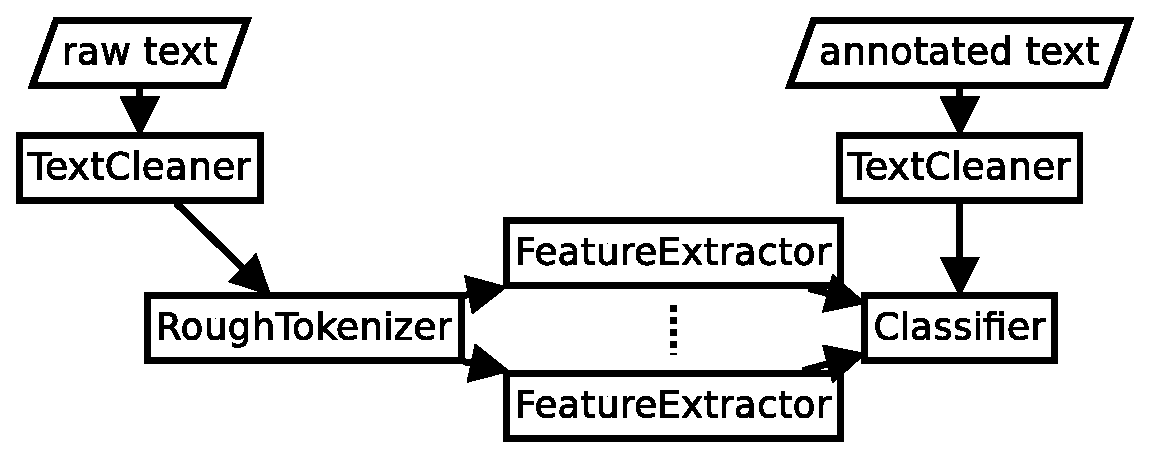
\includegraphics[width=\textwidth]{img/train-parts.eps}
  \caption{Data flow of the system in the training and evaluation
           configurations}
  \label{fig:train-parts}
\end{figure}

There is no output processing in the training mode as the only output produced,
apart from the saved maxent model file, are warning messages about token and
sentence boundaries found in the annotated version which are not even marked as
potential boundaries in the raw input. This is a signal to the user that he
should perhaps modify the tokenization scheme to account for more possible
boundaries or to check his annotated data. The setup of the system can be seen
on Figure~\ref{fig:train-parts}.

\subsection{Tokenization}
\label{ssec:impl-modes-tokenize}

After a model has been trained, the tokenization mode becomes available. In
this mode the text is cleaned, converted into rough tokens and tagged with
properties. The \class{Classifier} has the trained model loaded and predicts
the outcome (sentence boundary, token boundary or no boundary) for every
decision point given its context. This outcome is used to resolve the
\maysplit{}, \mayjoin{} and \maybreaksentence{} ambiguities and the
disambiguation is stored in the relevant rough token's metadata. These
annotated tokens are then printed through the \class{OutputFormatter} and
encoded with the \class{Encoder}. See the setup of the system in this mode on
Figure~\ref{fig:tokenize-parts}.

\begin{figure}
  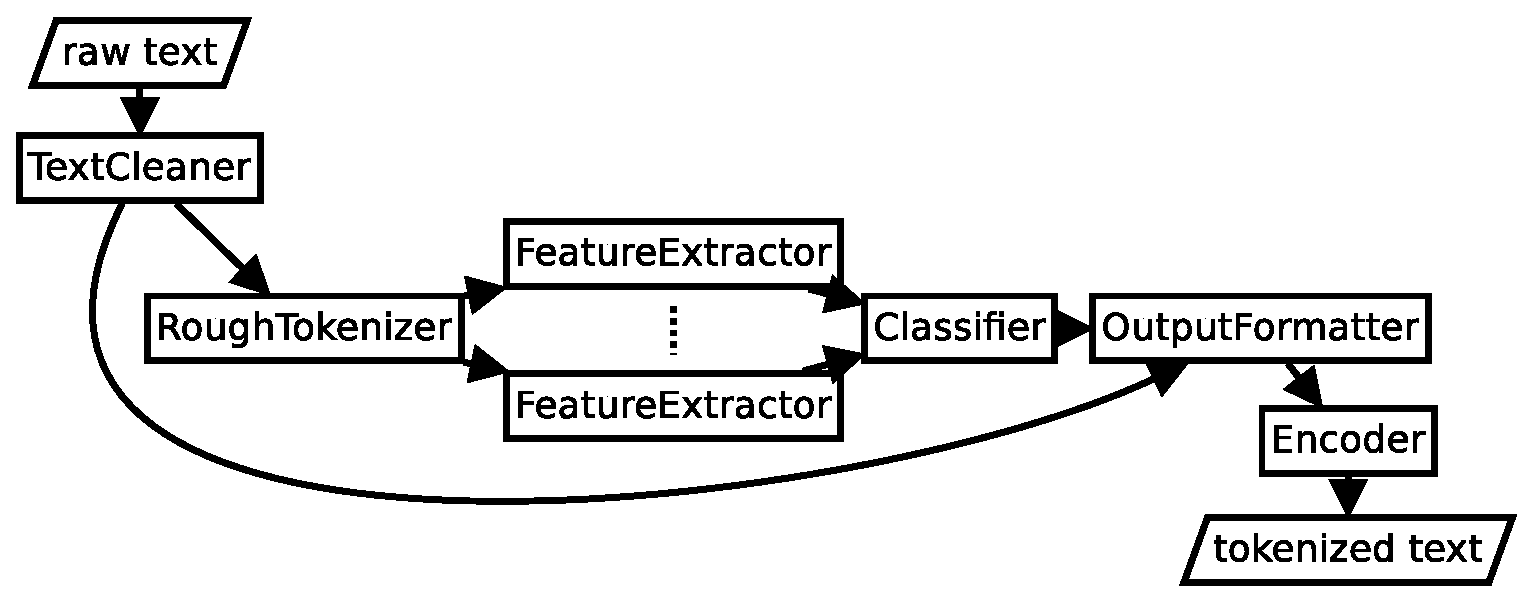
\includegraphics[width=\textwidth]{img/tokenize-parts.eps}
  \caption{Data flow of the system in the tokenization and preparation
           configurations}
  \label{fig:tokenize-parts}
\end{figure}

\subsection{Evaluation}
\label{ssec:impl-modes-evaluate}

When tweaking and developing a tokenization system (the selected training data,
the configured parameters in the tokenization scheme) it is vital to have
feedback on the shortcomings of your system. The evaluation mode was designed
just for this purpose. It works in a way similar to the training mode (see
Figure~\ref{fig:train-parts}). The \class{Classifier} aligns the rough tokens
with the annotated text and extracts the contextual properties from the tokens
and the true outcome from the annotated data. However, instead of recording
them it uses an already trained model and queries it for its predicted outcome.
The tokenizer then outputs both the true and the predicted outcome along with
the contextual properties.

Another tool can then be used to analyze the tokenizer's output and examine the
results and errors of the trained model. An example of such a tool would be the
included Python script analyze.py, which scans the evaluation's output and
reports the accuracy, precision, recall and F-measure of both sentence and
token boundary detection.

This log of outcomes and contexts can be written out when using any of the
available modes but only the evaluation mode has access to both the true
outcomes from the annotated data and the outcomes predicted by the
probabilistic model.

\subsection{Preparation}
\label{ssec:impl-modes-prepare}

The preparation is the last and least essential mode of the tokenizer. It is
similar to the tokenization mode (see Figure~\ref{fig:tokenize-parts}), but
instead of querying the probabilistic model for an outcome, the
\class{Classifier} simply confirms all potential boundaries (\maysplit{}
becomes a token boundary and \maybreaksentence{} becomes a sentence boundary).
This produces a file in which an annotator only has to remove spaces and line
breaks where inappropriate to get the correct annotation.

An advantage to using this mode might be that when the user does not demand the
logging of contexts as in the evaluation mode, the time-costly
\class{FeatureExtractor} and \class{Classifier} can be replaced with a
\class{SimplePreparer}, which only removes the ambiguities in the
abovementioned way.

\section{Rough Tokenization}
\label{sec:impl-roughtok}

One of the first problems encountered when designing the tokenizer was the
implementation of rough tokenization. The task of rough tokenization is to take
the definitions of decision points and then to be able to detect all such points
in any given input.

The possible positions for a \maysplit{} decision point are defined by pairs of
regular expressions: a position is to be marked as a \maysplit{} point if and
only if the first expression (prefix) matches some of the characters
leading to the position and the second expression (suffix) matches some of
the characters following it. \mayjoin{} decision points are defined almost the
same way, except that the characters following the position of a \mayjoin{}
must start with a string of blank characters and then continue with the string
matched by the regular expression. \maybreaksentence{} points, on the other
hand, are defined simply by two sets of characters. If a position follows a
character from the first set or precedes a character from the second set, then
that position is a \maybreaksentence{}. See Figure \ref{fig:decision-points} for an example.

\begin{figure}
  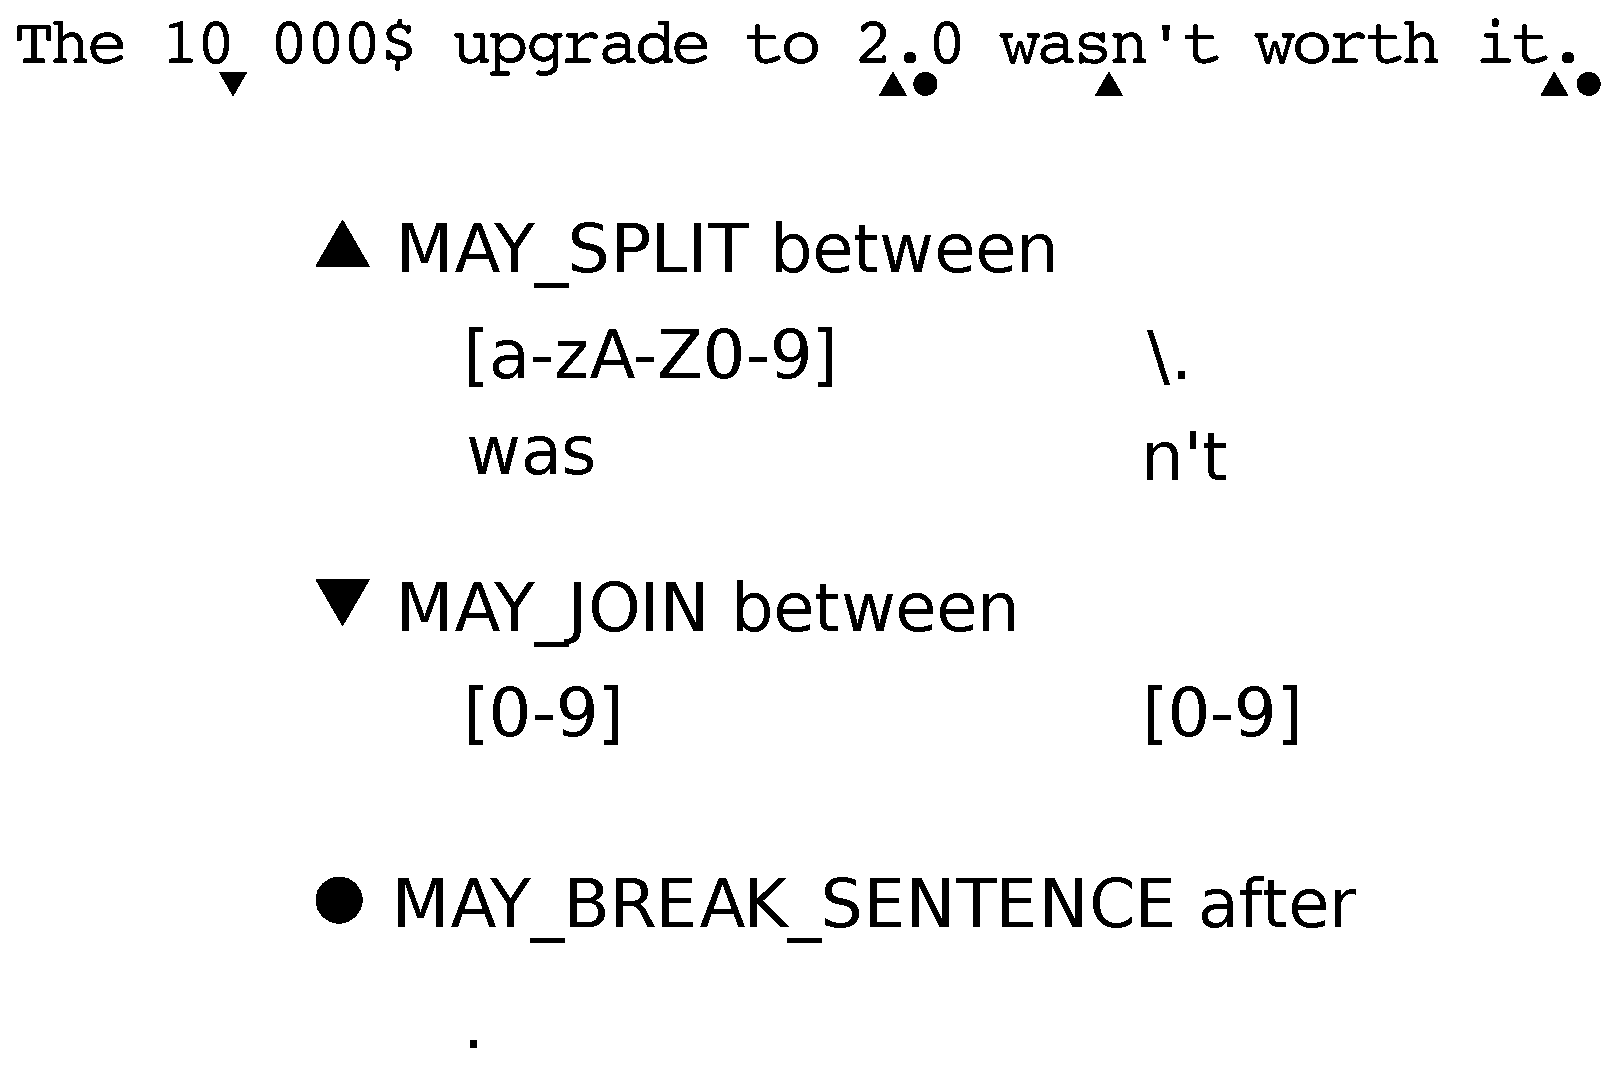
\includegraphics[width=0.618033988\textwidth]{img/decisionpoints.eps}
  \caption{An example sentence marked with demonstratory decision points. The
           definition of the decision point placement is described below the
           sentence. The sitting wedge triangle represents a \maysplit{}, the
           upside triangle marks a \mayjoin{}s and a circle marks the
           \maybreaksentence{} positions. The whitespace and the decision
           points divide the text into rough tokens.}
  \label{fig:decision-points}
\end{figure}


\subsection{Regular Expression Libraries}
\label{ssec:impl-roughtok-regex}

The reference implementation of the trainable tokenizer written in Perl used a
disjunction regular expression to match the prefix of the unprocessed input.
Our original idea was to use PCRE \cite{web-pcre} or some other regular expression
implementation \cite{web-boost,web-re2} to write a similar algorithm.

The naive approach might have us trying to search for the possible suffixes of
\mayjoin{}s and \maysplit{}s which are preceded by their respective prefixes.
Soon we would learn that finding one decision point may lock us out of finding
another one. For example, given the string \example{abcd} and \maysplit{}
regular expression pairs \example{a} - \example{bc} and \example{b} -
\example{c}, we match the \example{bc} according to the leftmost longest match
convention properly registering the \maysplit{} between \example{a} and
\example{bc}, but we lose the opportunity to find the \maysplit{} between
\example{b} and \example{c}.

If we try to search for each of these pairs of regular expressions
individually, we might still miss some points as demonstrated by the following
example. Let the string in question be \example{abab} and the \maysplit{}
regular expression pair \example{a} - \example{b(ab)*}. Any attempt to search
for the suffix \example{b(ab)*} would yield the \example{bab} substring due to
the leftmost longest match convention (and never just the final \example{b},
which means that position will not trigger a \maysplit). There are solutions to
this problem such as modifying the user's regular expression, modifyng the
regular expression matching function or searching for the suffix from every
position in the text, but they are all either difficult or ineffective.

We do not want to be patching the user's regular expressions because we would
probably have to restrict ourselves to a narrower set of regular expressions
and even then it would have been challenging to actually implement such a system
and prove its correctness. Writing our own regular expression matching engine
is also out of the scope of this work. The third option on the list, searching
for the suffix (or prefix) from every position in the text, seems like a
performance killer. Performance-wise speaking, during the planning phase of
development, prototypes of the naive method of regular expression rough
tokenization were implemented using both Boost.Regex and PCRE. The average
time spent on a 10 MB file with a credible set of splitting and joining rules
(breaking English contractions apart, separating words from punctuation
etc...) was over 10.8 seconds for Boost.Regex and over 4.9 seconds using
PCRE. The test were performed on a development laptop with the Intel Core 2
Duo T7500 processor.

\subsection{Lexical Analyzer Generators}
\label{ssec:impl-roughtok-lexergen}

During the initial planning, there was another radically different proposal for
handling rough tokenization which motivated the early prototypes.

The goal of rough tokenization is to scan large volumes of text and detect
patterns described by regular expressions. This kind of problem has been
already solved many times using lexical analyzer generators such as flex. These
tools take rules, which are pairs of regular expressions and actions written as
code. The lexical analyzer generator then creates a program from these rules
which reads a stream of text and tries to match a prefix of the yet unmatched
input with these regular expressions and reacts to the matches with the
supplied actions. More advanced tools enable the definition of several analyzer
modes with different rules and enables the actions to switch between them.

The lexical analyzer generator selected for our tokenizer was Quex
\cite{web-quex}. Its most important feature is that it is able to work on
Unicode code points instead of single-byte characters and that it uses libiconv
and ICU to process text in any encoding. Quex can also be very fast because it
does not encode the resulting automaton into a table which drives some general
program, but instead it generates low level C++ code which mimics the behaviour
of the automaton.

The naive way of rough tokenization presented in
subsection~\ref{ssec:impl-roughtok-regex} was implemented in a prototype to
evaluate the performance benefits stemming from the use of compiled lexers
generated by Quex. When run with the same tokenization rules and on the same
data as the rough tokenizers in subsection~\ref{ssec:impl-roughtok-regex}, the
Quex generated lexer finished on average in a little over 0.9 seconds. But the
generated lexer was making the same mistakes as the first approaches using
regular expressions. As we grew to know more of the functionality available to
us in Quex and the specifics of its operation, we were able to arrive at a
lexer which detects every possible decision point and does so in about 1.9
seconds on the same data set with which we tested the other methods. The
details of this final method are presented in
subsection~\ref{ssec:impl-roughtok-solution}.

\subsection{The Solution}
\label{ssec:impl-roughtok-solution}

\begin{figure}
  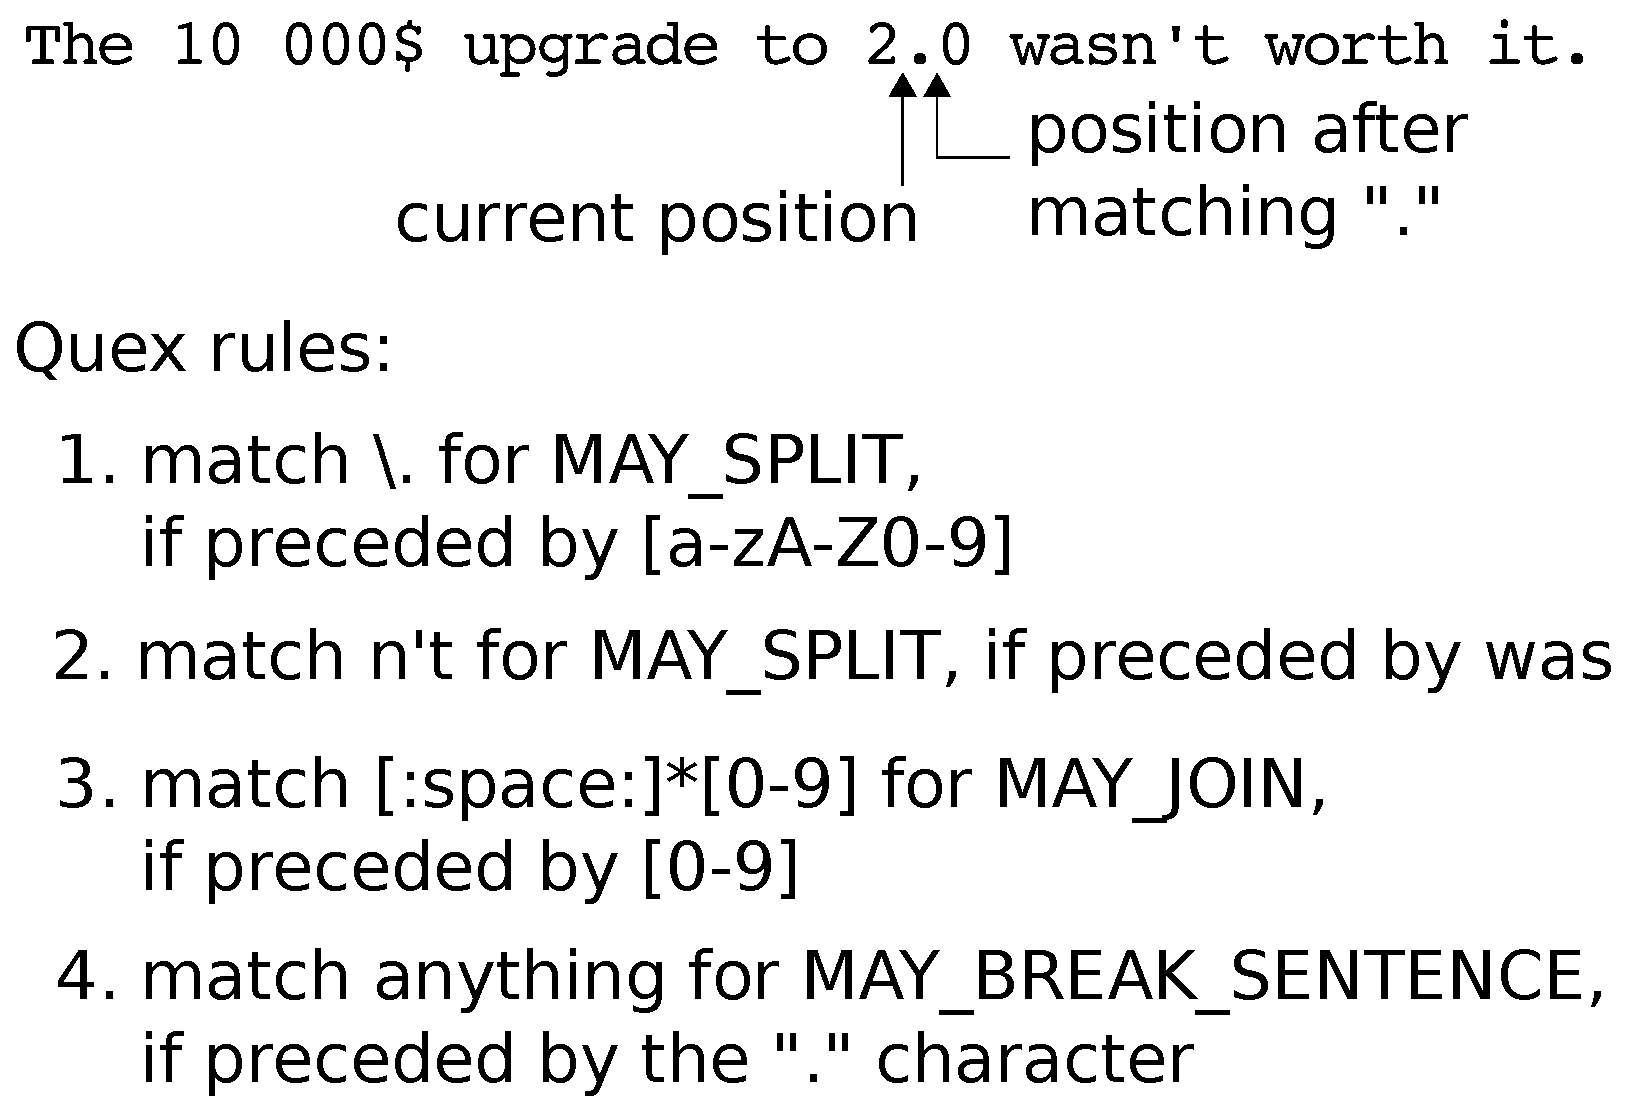
\includegraphics[width=0.618033988\textwidth]{img/quexexample.eps}
  \caption{An example of real-world implemented rough tokenization. The
  generated Quex lexer is at the signified position in the input. Given its
  position, the lexer takes into consideration only rules 1 and 3, as these are
  the only rules whose preconditions have been met. Rule 1 can match the
  input at the current position and so a \maysplit{} is announced and the
  word read so far ("2") is reported as a rough token. The lexer now
  automatically advances by the length of the matched string, but we manually
  step back to the original position in hope of finding more decision points
  at the current position and the positions within the matched string. When no
  further decision points are to be found at the current location (as is the
  case here), we move one character ahead.}
  \label{fig:quex-example}
\end{figure}

Many of the observations about the task at hand made in
subsection~\ref{ssec:impl-roughtok-regex} still hold when designing a Quex
generated lexer. The final implementation processes the input one character at
a time. At each position in the text, rules for matching the suffixes of
possible \maysplit{}s and \mayjoin{}s are in play. Each of these rules has a
condition in Quex that the preceding text must match the prefix of the
respective \maysplit{} or \mayjoin{} rule. The \maybreaksentence{} rules
are implemented in a similar way as their definitions are basically
specializations of the \maysplit{} and \mayjoin{} definitions (single
characters for prefix or suffix instead of regular expressions). An example of
such Quex rules can be seen on Figure~\ref{fig:quex-example}.

When the lexer matches the suffix of a decision point rule, it sends the last
characters read since the last decision point or whitespace as a rough token
and signals the decision point. Quex would now automatically advance our
position in the text right behind the matched suffix, but we override this
behaviour and move back to the position of the newly found decision point so
other decision points may be found. This alone would cause an infinite loop and
so upon returning to the original position we also scratch the detected
decision point from the set of applicable rules. If another decision point is
found, we do the same until we find all types of decision points at the current
location or none of the rules match anymore. In that case, the lowest priority
action takes place which reads another character from the stream and starts
looking for decision points at the next position.

This scratching out of rules is implemented using 8 different modes for all the
different sets of decision points we might be looking for. We start at the
topmost mode where we are looking for any of the 3 possible decision points. If
one of them is found, we continue at the same location in a mode which looks
for the remaining 2 possible decision points. In the final implementation,
there is also a demand for unexpanded HTML entities to be treated as single
rough tokens. This demand is met by adding another variable to the state of
the lexer (whether we are about to read an entity) which results in the 16
modes seen in the current implementation.

TODO: > K sekci 3.3.3: Stalo by za to zminit se o slozitosti, protoze je
kvadraticka
> v maximalni delce namatchovaneho suffixu, ne? Cili doopravdicka horni mez
> pro uplne pitoma pravidla je O(n\^2), ale v realu to bude jen
> n*mala\_konstanta.

Přesně tak to je, někde to do sekce 3.3.3 přidám.

\subsection{Technical Implementation}
\label{ssec:impl-roughtok-technical}

In the finished application, the regular expressions which define the placement
of decision points are read from user-written configuration files. A Quex
source file containing modes for detecting all of the decision points
referenced by the user is then output to a temporary file. CMake
\cite{web-cmake} is invoked to probe the user's system for the compiling
essentials, to generate a project for the user's preferred build system and to
write the command needed to start the build to a file. This file is read and
the command within it is run, which executes Quex on the generated source file
and then compiles the result into a shared module. This process is therefore
platform-agnostic as it doesn't rely on a specific C++ compiler or build system
and uses only CMake and Quex which are multiplatform and are required to build
the tokenizer itself.

This compiled shared module is then loaded using the libtool's dynamic loading
library \cite{web-libtool} which is a wrapper for the platform-specific dynamic
loading functions. The tokenizer tracks the set of files used to generate the
rough tokenizer along with their timestamps and only regenerates and recompiles
it when changes have been made.

\section{TODO: Classifier}

TODO:Na tom místě by pak stály dva rozhodovací body, což je pro tokenizér
standardní situace. Někam do kapitoly o implementaci bych asi ještě připsal
něco o tom, jak jsou rysy posbírány z okolí kontextu a spolu s rozhodovacími
body a jejich příp. rozřešeními jsou poslány klasifikátoru. V této implementaci
nejsou rozhodovací body tvořené vlastními tokeny, ale jsou to vlastnosti tokenů
(n-tý token má vlastnost \%\maysplit{} pokud mezi n-tý a n+1-ním je rozhodovací
bod \maysplit{}). Tím pádem pak tokenizér dezambiguuje všechny rozhodovací body
na dané pozici (vrací jeden ze tří výsledků: NOBOUNDARY, TOKENBOUNDARY nebo
SENTENCEBOUNDARY, podle něj se pak z \maysplit{} může stát DOSPLIT apod.).


\section{Parallelism}
\label{sec:impl-parallel}

One of the explicit goals when developing the tokenizer was performance.
However, apart from the rough tokenization and the probing of the tokens'
properties (the user-defined regular expressions and token lists), the
algorithms were quite straightforward. What could be tweaked, however, was the
manner of their implementation and execution. 

When the task of rough tokenization was isolated from the problem of
classifying the potential token and sentence boundaries, a producer/consumer
pattern was proposed to process both tasks in parallel. As the design of the
system became more detailed, more of the tasks became isolated and the original
idea of a producer/consumer pattern changed into the pipeline model seen in the
current implementation. Deciding on the pipeline model also let us use
libraries which offered high-level pipeline implementations. This meant we did
not have to implement the entire system from scratch using threads and
synchronization primitives. For the performance payoff of multi-threading, see
Chapter~\ref{chap:eval}

\subsection{The Pipeline}
\label{ssec:impl-parallel-pipeline}

Threading Building Blocks \cite{web-tbb}, an open-sourced library developed by
Intel, was used for implementing the pipeline. Compared to other mutliplatform
parallelism solutions, TBB offers high-level algorithms and constructs like the
pipeline. It also uses C++ classes and methods to expose its functionality
instead of relying on pragma directives like the standardized OpenMP
\cite{web-openmp}. 

The pipeline is constructed by setting up an array of filter objects. Each of
the filter objects must override the invocation operator and must identify
itself as either a parallel or a serial filter (parallel meaning that this
filter can be run simultaneously on multiple points of data, serial meaning
that the filter processes the input one at a time). In the tokenizer, the
\class{RoughTokenizer}, the \class{FeatureExtractor}, the \class{Classifier}
and the \class{OutputFormatter} are all elements of this pipeline (you can see
the pipeline as the middle row in Figure~\ref{fig:all-parts} with
\class{FeatureExtractor} being a parallel filter). The TBB library invokes the
first filter, the \class{RoughTokenizer}, and passes its return value to the
\class{FeatureExtractor} which also produces a value and so on...

Originally, the values to be flowing through the pipeline were individual rough
tokens, but the overhead would have been too big. The TBB library doesn't use
one thread per pipeline element, instead it is more similar to one thread per
value. This way the values are more likely to stay in the cache of the current
processor. So it was settled that chunks of rough tokens would be the work
units traversing the pipeline. Initially, the idea was to have them statically
sized, but since the \class{Classifier} can consume more tokens than it
produces and vice versa, the chunks are now dynamic (e.g.\ when processing the
first chunk, the \class{Classifier} cannot annotate the final tokens as it has
to wait for the next chunk which will inform it about the postcontext of those
final tokens).

\subsection{The Input/Output Threads}
\label{ssec:impl-parallel-io}

Initially, the plan was for the pipeline to encapsulate all of the parts of the
system. However, it would have been cumbersome to implement the
\class{RoughTokenizer} so that it is a function which receives a chunk of text,
feeds it to the buffer of the generated lexer, tries to tokenize the incomplete
chunk of text and then send the retrieved tokens along. The C++ Standard
Library already offers a widely used and supported FIFO structure for
transmitting continuous text, the \class{std::iostream}. In its
\class{stringstream} incarnation, it allows one agent to write text to it using
the standard output operators of C++ and then later another agent can use the
standard input operators to read and parse its contents. Such a standard
mechanism would allow us to simply pass a pointer to this stream to the Quex
lexer as if it were a file handle and we would not have to trouble ourselves
with any string marshalling.

A class which does just this was implemented by Alexander Nasonov and published
on the Boost mailing list in 2003 \cite{web-pipes}. However, it didn't meet
with much understanding on the list as people tended to associate the class'
name, \class{pipe}, with OS-level pipes. The pipestreams have been resurrected
for this project and they made writing the transfer of text between the
\class{TextCleaner}, the \class{Encoder} and the parts of the TBB pipeline
very simple.

The pipestreams were used to connect the \class{TextCleaner} and
\class{Encoder} to the TBB pipeline. The \class{TextCleaner} and the
\class{Encoder} both have a do\_\-work method which does all the work. In the
case of the \class{TextCleaner}, it uses a Quex generated lexer to find XML
markup and entities in the input file. It optionally transforms these
segments, reports them to the \class{OutputFormatter} and writes the
transformed input to an \class{opipestream} (an output pipestream). The
\class{Encoder} on the other hand reads from an \class{ipipestream} (an input
pipestream), transcodes the text read and writes it to the output file. The
use of pipestreams to connect the TBB pipeline world with the I/O world might
also have a performance advantage, because TBB pipelines are not optimized for
I/O heavy operations and perform badly when stalling on I/O. These
input/output threads (those which run the do\_\-work methods) might decrease
the probability of a pipeline thread waiting for I/O by filling the pipestream
buffers while working on a different CPU.
